%%%%%%%%%%%%%%%%%%%%%%%%%%%%%%%%%%%%%%%%%%%%%%%%%%%%%%%%%%%%%%
%% Presentation template and short Beamer example/tutorial.
%% Vincent Labatut 2017-19 <vincent.labatut@univ-avignon.fr>
%%%%%%%%%%%%%%%%%%%%%%%%%%%%%%%%%%%%%%%%%%%%%%%%%%%%%%%%%%%%%%
% setup Beamer
\documentclass[10pt,    % default is 11pt, use 10pt for more compact slides
%    handout,            % collapse all overlays (=animations) and video-invert console text
    english,            % presentation language (theme supports only french & english)
    xcolor=table,       % colors in the tables
    envcountsect,       % include section number in theorem numbers
    aspectratio=43      % format: only 16:9 (169) and 4:3 (43) are supported
]{beamer}

%%%%%%%%%%%%%%%%%%%%%%%%%%%%%%%%%%%%%%%%%%%%%%%%%%%%%%%%%%%%%%
% setup the theme
% \usepackage{au/sty/beamerthemeAU}         % no option at all
\usepackage[light]{au/sty/beamerthemeAU}   % the "light" option only changes the title and section pages

%%%%%%%%%%%%%%%%%%%%%%%%%%%%%%%%%%%%%%%%%%%%%%%%%%%%%%%%%%%%%%
% setup side notes
\usepackage{pgfpages}                                   % comment all 3 below lines to hide notes
%\setbeameroption{show notes}                           % alternate content and note slides
%\setbeameroption{show only notes}                      % only note slides
%\setbeameroption{show notes on second screen=right}    % dualscreen: right, left, top, bottom

%%%%%%%%%%%%%%%%%%%%%%%%%%%%%%%%%%%%%%%%%%%%%%%%%%%%%%%%%%%%%%
% name of the biblatex file
\addbibresource{biblio.bib}







%%%%%%%%%%%%%%%%%%%%%%%%%%%%%%%%%%%%%%%%%%%%%%%%%%%%%%%%%%%%%%
% title and subtitle of the presentation (the latter is optional)
\title[Short Title] % leave empty for no title in footer
    {Here is a presentation with a very long title aiming at filling several lines in the title page}
\subtitle{It is also possible to define a relatively long subtitle such as this one} % leave empty if no subtitle
%%%%%%%%%%%%%%%%%%%%%%%%%%%%%%%%%%%%%%%%%%%%%%%%%%%%%%%%%%%%%%
% date of the presentation (leave empty for no date, default is today)
\date[Short date] % leave empty for no date in footer
    {\today}
%%%%%%%%%%%%%%%%%%%%%%%%%%%%%%%%%%%%%%%%%%%%%%%%%%%%%%%%%%%%%%
% authors and their affiliations (the latter is optional)
\author[Short author] % leave empty for no author in footer
{FirstnameA~LastnameA\inst{1} \and \underline{FirstnameB~LastnameB}\inst{2} \and FirstnameC~LastnameC\textsuperscript{1,2}}
\institute[] % (short affiliation not used in this theme)
{\inst{1} Computer Science Lab, Avignon University -- LIA EA 4128 \texttt{\{firstname.lastname\}@univ-avignon.fr}
\and \inst{2} Institute of Disruptive Innovation, University of Excellence \texttt{\{firstname.lastname\}@univ-excell.fr}
}
%%%%%%%%%%%%%%%%%%%%%%%%%%%%%%%%%%%%%%%%%%%%%%%%%%%%%%%%%%%%%%
% optional: additional logo (ex. lab)
\titlegraphic{
\includegraphics[width=3cm,]{images/lia_logo.pdf}}
% if you want several logos, put them in a box
% \titlegraphic{\parbox{3cm}{\hspace   {0.5cm}
\includegraphics[width=2.5cm,]{images/ceri_logo.pdf}\newline
\includegraphics[width=3cm,]{images/lia_logo.pdf}}}
%%%%%%%%%%%%%%%%%%%%%%%%%%%%%%%%%%%%%%%%%%%%%%%%%%%%%%%%%%%%%%









%%%%%%%%%%%%%%%%%%%%%%%%%%%%%%%%%%%%%%%%%%%%%%%%%%%%%%%%%%%%%%
\begin{document}
%%% title page
\begin{frame}
  \titlepage
\end{frame}

%%% presentation
\begin{frame}
    \label{frm:first}
    \frametitle{Presentation} 
    
    This is an unofficial adaptation of the official template of \href{http://univ-avignon.fr/}{Avignon Université}, originally proposed only in \href{https://en.wikipedia.org/wiki/Microsoft\_PowerPoint}{MS PowerPoint} and \href{https://en.wikipedia.org/wiki/LibreOffice\#Included\_applications}{LO Impress} formats at the following address (authentication required):
    
    \url{https://e-doc.univ-avignon.fr/maison-de-la-communication/charte-graphique-de-luniversite/}
    
    \vspace{0.25cm}
    This presentation file also illustrates how to use basic \href{https://en.wikipedia.org/wiki/Beamer_(LaTeX)}{Beamer} features, assuming the reader already knows how to use \LaTeX{}. A more complete (and general) \LaTeX{} tutorial (in French) can be found here: 
    
    \url{https://www.overleaf.com/latex/templates/modele-rapport-uapv/pdbgdpzsgwrt}
    
    It is also a report template for the same institution.
    
    \vspace{0.25cm}
    The \LaTeX{} source code contains additional details under the form of comments.
    
    \vspace{0.25cm}
    A French version of these slides can be produced by compiling \texttt{main\_FR.tex} instead of \texttt{main\_EN.tex}.
\end{frame}

%%% outline of the presentation
\begin{frame}{Outline}
    \tableofcontents
%        [hideallsubsections] % un-comment this line to hide sub-sections
\end{frame}












%%%%%%%%%%%%%%%%%%%%%%%%%%%%%%%%%%%%%%%%%%%%%%%%%%%%%%%%%%%%%%
\section{Basics Features}
\label{sec:basics}
\sectionframe

%%%%%%%%%%%%%%%%%%%%%%%%%%%%%%
\subsection{Class, Pages \& Sections}
%%%
\begin{frame}
    \frametitle{Beamer Class \& AU Theme}
    
    The original Beamer class takes a number of options, among which:
    \begin{itemize}
        \item \texttt{handout}: document rendered for printing (disables overlays, dark backgrounds, etc.);
        \item regular font size: default is \texttt{11pt};
    \end{itemize}

    \vspace{0.25cm}
    The AU Beamer theme proposed here, \texttt{beamerthemeAU}, also has an option \texttt{light}, which changes the background of the title and section pages.
    
    \vspace{0.25cm}
    The \textit{aspect ratio} of the slides can be controled through parameter \texttt{aspectratio}. This theme supports two options: \texttt{43} (4:3, the default value), and \texttt{169} (16:9).
\end{frame}

%%%
\begin{frame}
    \frametitle{Pages : It is possible to have long titles spanning two lines, like here} 
    
    In Beamer, one page of the presentation is called a \textit{frame}, and can be defined through the \texttt{frame} environment.
    
    \vspace{0.25cm}
    The title and subtitle of a page are set using the \texttt{\textbackslash{}title} and \texttt{\textbackslash{}subtitle} commands, respectively. The subtitle can be omitted, as in this page. See next page for an example of subtitle.
    
    \vspace{0.25cm}
    The \texttt{frame} environment has a number of options, including: 
    \begin{itemize}
        \item \texttt{plain}: to remove all decorations;
        \item \texttt{allowframebreaks}: to split automatically long content over several pages (eg. bibliography, Section~\ref{sec:biblio});
%        \item \texttt{shrink}: compact text for verbose pages; % this theme does not support this option
        \item \texttt{fragile}: when using verbatim environments (eg. \texttt{listings}, Page~\ref{frm:sourcecode});
        \item Vertical alignment: \texttt{c} (center), \texttt{t} (top) or \texttt{b} (bottom).
    \end{itemize}
\end{frame}

%%%
\begin{frame}
    \frametitle{Sections} 
    \framesubtitle{It is possible to add a subtitle below the title, which can also span two lines if needed}
    
    Sections and subsections are handled like in regular \LaTeX{} documents, i.e. using the \texttt{\textbackslash{}section} and \texttt{\textbackslash{}subsection} commands, respectively.
    
    \vspace{0.25cm}
    Using the command \texttt{\textbackslash{}tableofcontents}, it is possible to automatically fill a page with the table of contents. The option \texttt{hideallsubsections} allows including only sections (and not subsections).
    
    \vspace{0.25cm}
    The command \texttt{\textbackslash{}sectionframe} can be used to insert a page containing only the title of the current section, eg. Section~\ref{sec:basics}.
\end{frame}




%%%%%%%%%%%%%%%%%%%%%%%%%%%%%%
\subsection{Text Formatting}
%%%
\begin{frame}
    \frametitle{Text Formatting} 
    \framesubtitle{Standard Commands} 
    
    Like in regular \LaTeX{} documents, it is possible to define \textit{italic} (\texttt{\textbackslash{}textit}) or \textbf{bold} (\texttt{\textbackslash{}textbf}) text, or \textit{\textbf{both}} (by combining these commands). 
    
    \vspace{0.25cm}
    One can also use a \texttt{monospaced} font (\texttt{\textbackslash{}texttt}).
    
    \vspace{0.25cm}
    It is also possible to use the \texttt{\textbackslash{}alert} command, which is specific to Beamer, in order to add some color, like here: \alert{Alert!}
    
    % paragraphs
    % to leave space between paragraphs: \smallskip, \medskip, & \bigskip 
\end{frame}
    
%%%
\begin{frame}
    \frametitle{Text Formatting} 
    \framesubtitle{Theme-Specific Commands} 
    
    Command \texttt{\textbackslash{}textsc}, which allows formatting the text using smaller upper-case letters (a.k.a. \textit{small caps}) has no effect, because the font used by the theme does not support small caps. However, the theme proposes command \texttt{\textbackslash{}fauxsc} in order to simulate this effect: \fauxsc{This is how the text looks like when using this command}.
    
    \vspace{0.25cm}
    The middle dot used in French for gender-inclusive writting can be obtained thanks to command \texttt{\textbackslash{}textperiodcentered}, or the shorter \texttt{\textbackslash{}tpc}. For instance: chercheur\textperiodcentered{}se\tpc{}s. The user can alternatively directly insert the character by copying and pasting this instance: ``·''.

    \vspace{0.25cm}
    The theme contains commands for matching \textit{check} and \textit{cross marks}: \cmark{} (\texttt{\textbackslash{}cmark\{\}}) and \xmark{} (\texttt{\textbackslash{}xmark\{\}}).
\end{frame}
    
%%%
\begin{frame}
    \frametitle{Quotations}
    
    One can quote text using the \texttt{verse} environment, e.g.
    \begin{verse}
        Quotation, n: The act of repeating erroneously the words of another. \\ 
        \vspace{-0.5cm}
        \begin{flushright}--A. Bierce\end{flushright}
    \end{verse}
    
    Or the \texttt{quote} environment:
    \begin{quote}
        Build a man a fire, and he'll be warm for a day. Set a man on fire, and he'll be warm for the rest of his life. \\ 
        \begin{flushright}--T. Pratchett\end{flushright}
    \end{quote}
\end{frame}
    
%%%
\begin{frame}
    \frametitle{Mathematical Expressions} 
    
    \textit{In-line} equations are defined with \texttt{\$}, e.g. \texttt{\$f(x) = ax + b\$} is rendered as $f(x)=ax + b$.
    
    \vspace{0.25cm}
    \textit{Off-line} equations, which are numbered, are inserted using the \texttt{equation} environment, e.g.
    \begin{equation}
        \label{equ:affine}
        f(x) = ax + b.
    \end{equation}
    
    Command \texttt{\textbackslash{}nonumber} prevents the numbering of the off-line equations, e.g.
    \begin{equation}
        \label{equ:rayleigh}
        r(\mathbf{x},\mathbf{M}) = \frac{\mathbf{x}^\top \mathbf{M} \mathbf{x}}{\mathbf{x}^\top \mathbf{x}}. \nonumber
    \end{equation}
    
    % Binomial coefficient:
    % \binom{n}{k}
    
    % Parentheses:
    %   Sizes: \big \Big \bigg \Bigg
    %   Types: ( ) [ ] \langle \rangle | \|
    %
    %   See: https://www.overleaf.com/learn/latex/Brackets_and_Parentheses
    
    % Symbols
    %   Empty set: \varnothing
    %
    %   See: https://oeis.org/wiki/List_of_LaTeX_mathematical_symbols
    
    % Formatting
    % Field: \mathbb{}
    % Gras: \mathbf{}
    % Caligraphed: \mathcal{}
    
    % Cases
    %   \begin{cases}
    %       1 & \text{if } x > 3 \\
    %       0 & \text{otherwise}
    %   \end{cases}
    
    % Style
    % Offline: \displaystyle
    % Online: \textstyle
    % Tight: \scriptstyle
    % Tighter: \scriptscriptstyle
\end{frame}




%%%%%%%%%%%%%%%%%%%%%%%%%%%%%%
\subsection{Columns, Blocks \& Lists}
%%%%
\begin{frame}
    \frametitle{Columns}
    
    \begin{columns}[T,totalwidth=\textwidth] % 
        \begin{column}{0.33\textwidth}
            Using the \texttt{columns} and \texttt{column} environments (cf. this page's source code), it is possible to split a page in several independent columns. 
            
            This can ease defining the structure of the page.
        \end{column}
        
        \begin{column}{0.33\textwidth}
            For \texttt{columns}, options \texttt{t}, \texttt{b}, \texttt{c}, \texttt{T} control the vertical alignment, and \texttt{totalwidth} the global width (see \href{https://tex.stackexchange.com/a/51509/31360}{this page} for more details).
            
            The width of each column can be specified through the parameter of \texttt{column}.
        \end{column}
        
        \begin{column}{0.33\textwidth}
            It is possible to put text, but also images in columns.
            \begin{figure}[H]
                \centering
                % for some XeTeX-related reason, it is necessary to use the \XeTeXLinkBox command when associating a hyperlink to an image
                \href{http://univ-avignon.fr}{\XeTeXLinkBox{
\includegraphics[scale=1]{au/backgrounds/au_col_logo.pdf}}}
                \vspace{-0.5cm}
                \caption{Logo of Avignon Université}
                \label{fig:AUlogo}
            \end{figure}
        \end{column}
    \end{columns}

    % % empty column template
    % \begin{columns}[T,totalwidth=\textwidth] % 
    %     \begin{column}{0.5\textwidth}
    %         xxxx
    %     \end{column}
        
    %     \begin{column}{0.5\textwidth}
    %         xxxx
    %     \end{column}
    % \end{columns}
\end{frame}

%%%%
\begin{frame}
    \frametitle{Blocks}
    \label{frm:blocks}
    
    Blocks are specific to Beamer, and allow highlighting points of interest. There are three types of blocks, each one withi its own colors:

    \begin{block}{Regular}
        \texttt{block} environment: used most of the time.
    \end{block}

    \begin{alertblock}{Alert}
        \texttt{alertblock} environment: to highlight particularly important points.
    \end{alertblock}

    \begin{exampleblock}{\smaller[2] Example}
        \smaller[2]
        \texttt{exampleblock} environment: to show some concrete illustrations of the presented concepts.
    \end{exampleblock}
    
    One can reduce block size by using commands changing the font size, e.g. \texttt{\textbackslash{}smaller[2]}, as above with the example block (see source code).
    
    in order to center a formula in a block
    % \begin{block}{My block}
    %     My formula is:
        
    %     \centering 
    %     $y = ax + b$,
    
    %     \raggedright
    %     and here is the rest of the text.
    % \end{block}
    
    % or just use an equation environment
    
    % convenient commands
    % bar on top of some expression: \overline (betterm than \bar)
    % list of math symbols: https://oeis.org/wiki/List_of_LaTeX_mathematical_symbols
\end{frame}

%%%%
\begin{frame}
    \frametitle{Lists}
    
    Lists are defined as in \LaTeX{} documents, using the \texttt{\textbackslash{}item} command and one of the three existing environments:
    \begin{columns}[T,onlytextwidth]
        \begin{column}{0.33\textwidth}
            \texttt{itemize}:
            \begin{itemize}
                \item Rock;
                \begin{itemize}
                    \item Paper;
                    \begin{itemize}
                        \item Scissors.
                    \end{itemize}
                \end{itemize}
            \end{itemize}
        \end{column}
        \begin{column}{0.33\textwidth}
            \texttt{enumerate}:
            \begin{enumerate}
                \item First;
                \begin{enumerate}
                    \item Second;
                    \begin{enumerate}
                        \item Third.
                    \end{enumerate}
                \end{enumerate}
            \end{enumerate}
        \end{column}
        \begin{column}{0.33\textwidth}
            \texttt{description}:
            \begin{description}
                \item[Yin] Yang.
                \item[Hot] Cold.
            \end{description}
        \end{column}
    \end{columns}
    
    % to control the space between the list items
    % \begin{itemize}
    %     \setlength{\itemsep}{-0.1cm}    % for the first level only, must be repeated at each level
    %     \item Bla bla bla.
    % \end{itemize}
    
    % to change the starting number in a numbered list
    % \begin{enumerate}
    %       \setcounter{enumi}{3}    % the list will start at number 4
    %     \item Bla bla bla.
    % \end{enumerate}
    
    \vspace{0.25cm}
    Note the use of the \texttt{columns} and \texttt{column} environments in this page.
\end{frame}



%%%%%%%%%%%%%%%%%%%%%%%%%%%%%%
\subsection{Side Notes}
%%%%
\begin{frame}
    \frametitle{Side Notes}
    \framesubtitle{Defining Notes}
    
    It is possible to associate textual notes to each slide, using the \texttt{\textbackslash{}note} command and specifying a comment as parameter. Notes can be defined:
    \note{This is a note. It appears first in the corresponding text slide. }
    \begin{itemize}
        \item \textit{Inside} a \texttt{frame} environment: all notes contained in the same frame are gathered on the same text slide.
        \note[item]{This note appears as an item in a list placed at the end of the text slide.}
        \item \textit{Outside} frames: each note constitutes a single text slide.
    \end{itemize}
    \note{This note appears second. }
    
    \vspace{0.25cm}
    \note[item]{This is a second item in the list.}
    The \texttt{\textbackslash{}note} command has two options \texttt{item} (inside frames) and \texttt{itemize} (outside), both allowing to automatically organize comments as a list in the produced text slide. See the notes associated to this page.
    \note[item]{And a third list item.}
    \note{We finish with this comment, which will be placed \textit{before} the list. Note that notes are compatible with overlays, see Section~\ref{sec:animations}.}
\end{frame}

%%%%
\begin{frame}   
    \label{frm:dispnotes}
    \frametitle{Side Notes}
    \framesubtitle{Displaying Notes}
        
    \vspace{0.25cm}
    A number of Beamer options allow controlling how notes are shown:
    \begin{itemize}
        \item \texttt{hide notes} (default): notes are not shown in the slides.
        \item \texttt{show notes}: shows notes in additional text slides inserted between regular slides.
        \item \texttt{show only notes}: shows only these additional text slides, and not the regular ones.
        \item \texttt{show notes on second screen=right} (or \texttt{left}, \texttt{top}, \texttt{bottom}): take advantage of package \href{https://ctan.org/pkg/pdfpages?lang=en}{\texttt{pgfpages}} to enlarge the slides so that notes can be shown on a second screen (and therefore hidden to the audience). An appropriate software is then required to display the presentation, such as \href{http://impressive.sourceforge.net/}{Impress!ve} or \href{http://dspdfviewer.danny-edel.de/}{Dual-Screen PDF Viewer}.
    \end{itemize}
    
    \textbf{Note:} You can show the notes associated to the previous slide by setting the option accordingly at the begining of this document.
\end{frame}











%%%%%%%%%%%%%%%%%%%%%%%%%%%%%%%%%%%%%%%%%%%%%%%%%%%%%%%%%%%%%%
\section{Floats \& Cross-References}
\sectionframe

%%%%%%%%%%%%%%%%%%%%%%%%%%%%%%
\subsection{Figures \& Tables}
%%%%
\begin{frame}
    \frametitle{Figures}
    
    Figures can be inserted using the \texttt{figure} environment, as in regular \LaTeX{} documents.
    
    \begin{figure}[H]
        \centering
        
\includegraphics[scale=0.05]{images/lia_logo.pdf}
        \vspace{-0.5cm}
        \caption{Logo of the Computer Science Lab of Avignon Université}
        \label{fig:LIAlogo}
    \end{figure}
    
    \vspace{0.25cm}
    For an image stored in a \textit{file} (JPEG, BMP, PDF, PNG, etc.), as above, one uses the \texttt{\textbackslash{}includegraphics} command.
    
    % vertical bar to separate side-by-side figures  (see p.\label{sli:Diagrammes} for an example)
    % \rulesep

    % To define the position of a figure using absolute coordinates:
    % \begin{tikzpicture}[remember picture,overlay]
    %     \node[xshift=0cm,yshift=-1.5cm] at (current page.center) {\resizebox{0.8\linewidth}{!}{\input{images/02/shakespeare_inter.tex}}};
    % \end{tikzpicture}
    % see also: https://tex.stackexchange.com/a/89592/31360
\end{frame}

%%%%
\begin{frame}
    \label{sli:Diagrams}
    \frametitle{Diagrams}
    Besides image files, it is also possible to insert \textit{diagrams} into figures, thanks to the \href{https://ctan.org/pkg/pgf?lang=en}{\texttt{TikZ}} package:

    \vspace{-0.20cm}
    \begin{figure}[H]
        \centering
        \resizebox{0.35\linewidth}{!}{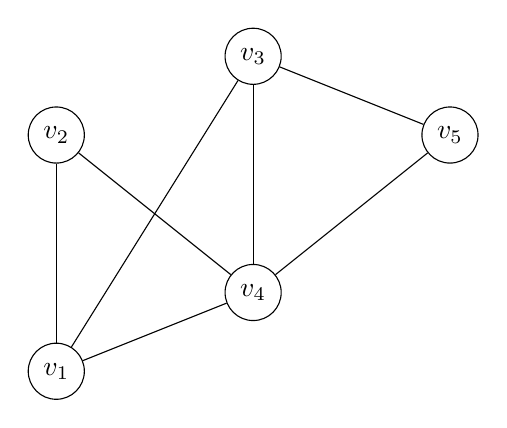
\begin{tikzpicture}
    % insert nodes
    \node[shape=circle,draw=black] (v1) at (0,0) {$v_1$};
    \node[shape=circle,draw=black] (v2) at (0,3) {$v_2$};
    \node[shape=circle,draw=black] (v3) at (2.5,4) {$v_3$};
    \node[shape=circle,draw=black] (v4) at (2.5,1) {$v_4$};
    \node[shape=circle,draw=black] (v5) at (5,3) {$v_5$} ;
    
    % insert links
	\draw (v1) -- (v2);
    \draw (v1) -- (v4);
	\draw (v1) -- (v3);
    \draw (v4) -- (v5);
    \draw (v3) -- (v4);
    \draw (v4) -- (v2);
    \draw (v5) -- (v3);
\end{tikzpicture}
}
        \hspace{0.25cm}\rulesep\hspace{0.25cm}
        \resizebox{0.45\linewidth}{!}{% Graphic for TeX using PGF
% Title: C:\Users\Vincent\Downloads\classdiag.dia
% Creator: Dia v0.97.2
% CreationDate: Mon Sep 24 11:08:38 2018
% For: Vincent
% \usepackage{tikz}
% The following commands are not supported in PSTricks at present
% We define them conditionally, so when they are implemented,
% this pgf file will use them.
\ifx\du\undefined
  \newlength{\du}
\fi
\setlength{\du}{15\unitlength}
\begin{tikzpicture}
\pgftransformxscale{1.000000}
\pgftransformyscale{-1.000000}
\definecolor{dialinecolor}{rgb}{0.000000, 0.000000, 0.000000}
\pgfsetstrokecolor{dialinecolor}
\definecolor{dialinecolor}{rgb}{1.000000, 1.000000, 1.000000}
\pgfsetfillcolor{dialinecolor}
\pgfsetlinewidth{0.100000\du}
\pgfsetdash{}{0pt}
\definecolor{dialinecolor}{rgb}{1.000000, 1.000000, 1.000000}
\pgfsetfillcolor{dialinecolor}
\fill (34.325000\du,11.850000\du)--(34.325000\du,13.250000\du)--(41.370000\du,13.250000\du)--(41.370000\du,11.850000\du)--cycle;
\definecolor{dialinecolor}{rgb}{0.000000, 0.000000, 0.000000}
\pgfsetstrokecolor{dialinecolor}
\draw (34.325000\du,11.850000\du)--(34.325000\du,13.250000\du)--(41.370000\du,13.250000\du)--(41.370000\du,11.850000\du)--cycle;
% setfont left to latex
\definecolor{dialinecolor}{rgb}{0.000000, 0.000000, 0.000000}
\pgfsetstrokecolor{dialinecolor}
\node at (37.847500\du,12.800000\du){Student};
\definecolor{dialinecolor}{rgb}{1.000000, 1.000000, 1.000000}
\pgfsetfillcolor{dialinecolor}
\fill (34.325000\du,13.250000\du)--(34.325000\du,16.650000\du)--(41.370000\du,16.650000\du)--(41.370000\du,13.250000\du)--cycle;
\definecolor{dialinecolor}{rgb}{0.000000, 0.000000, 0.000000}
\pgfsetstrokecolor{dialinecolor}
\draw (34.325000\du,13.250000\du)--(34.325000\du,16.650000\du)--(41.370000\du,16.650000\du)--(41.370000\du,13.250000\du)--cycle;
% setfont left to latex
\definecolor{dialinecolor}{rgb}{0.000000, 0.000000, 0.000000}
\pgfsetstrokecolor{dialinecolor}
\node[anchor=west] at (34.475000\du,13.950000\du){+name};
% setfont left to latex
\definecolor{dialinecolor}{rgb}{0.000000, 0.000000, 0.000000}
\pgfsetstrokecolor{dialinecolor}
\node[anchor=west] at (34.475000\du,14.750000\du){+firstname};
% setfont left to latex
\definecolor{dialinecolor}{rgb}{0.000000, 0.000000, 0.000000}
\pgfsetstrokecolor{dialinecolor}
\node[anchor=west] at (34.475000\du,15.550000\du){+age};
% setfont left to latex
\definecolor{dialinecolor}{rgb}{0.000000, 0.000000, 0.000000}
\pgfsetstrokecolor{dialinecolor}
\node[anchor=west] at (34.475000\du,16.350000\du){+gender};
\definecolor{dialinecolor}{rgb}{1.000000, 1.000000, 1.000000}
\pgfsetfillcolor{dialinecolor}
\fill (34.325000\du,16.650000\du)--(34.325000\du,17.650000\du)--(41.370000\du,17.650000\du)--(41.370000\du,16.650000\du)--cycle;
\definecolor{dialinecolor}{rgb}{0.000000, 0.000000, 0.000000}
\pgfsetstrokecolor{dialinecolor}
\draw (34.325000\du,16.650000\du)--(34.325000\du,17.650000\du)--(41.370000\du,17.650000\du)--(41.370000\du,16.650000\du)--cycle;
% setfont left to latex
\definecolor{dialinecolor}{rgb}{0.000000, 0.000000, 0.000000}
\pgfsetstrokecolor{dialinecolor}
\node[anchor=west] at (34.475000\du,17.350000\du){+register(course)};
\pgfsetlinewidth{0.100000\du}
\pgfsetdash{}{0pt}
\definecolor{dialinecolor}{rgb}{1.000000, 1.000000, 1.000000}
\pgfsetfillcolor{dialinecolor}
\fill (47.275000\du,16.750000\du)--(47.275000\du,18.150000\du)--(53.165000\du,18.150000\du)--(53.165000\du,16.750000\du)--cycle;
\definecolor{dialinecolor}{rgb}{0.000000, 0.000000, 0.000000}
\pgfsetstrokecolor{dialinecolor}
\draw (47.275000\du,16.750000\du)--(47.275000\du,18.150000\du)--(53.165000\du,18.150000\du)--(53.165000\du,16.750000\du)--cycle;
% setfont left to latex
\definecolor{dialinecolor}{rgb}{0.000000, 0.000000, 0.000000}
\pgfsetstrokecolor{dialinecolor}
\node at (50.220000\du,17.700000\du){Course};
\definecolor{dialinecolor}{rgb}{1.000000, 1.000000, 1.000000}
\pgfsetfillcolor{dialinecolor}
\fill (47.275000\du,18.150000\du)--(47.275000\du,19.950000\du)--(53.165000\du,19.950000\du)--(53.165000\du,18.150000\du)--cycle;
\definecolor{dialinecolor}{rgb}{0.000000, 0.000000, 0.000000}
\pgfsetstrokecolor{dialinecolor}
\draw (47.275000\du,18.150000\du)--(47.275000\du,19.950000\du)--(53.165000\du,19.950000\du)--(53.165000\du,18.150000\du)--cycle;
% setfont left to latex
\definecolor{dialinecolor}{rgb}{0.000000, 0.000000, 0.000000}
\pgfsetstrokecolor{dialinecolor}
\node[anchor=west] at (47.425000\du,18.850000\du){+name};
% setfont left to latex
\definecolor{dialinecolor}{rgb}{0.000000, 0.000000, 0.000000}
\pgfsetstrokecolor{dialinecolor}
\node[anchor=west] at (47.425000\du,19.650000\du){+year};
\definecolor{dialinecolor}{rgb}{1.000000, 1.000000, 1.000000}
\pgfsetfillcolor{dialinecolor}
\fill (47.275000\du,19.950000\du)--(47.275000\du,22.550000\du)--(53.165000\du,22.550000\du)--(53.165000\du,19.950000\du)--cycle;
\definecolor{dialinecolor}{rgb}{0.000000, 0.000000, 0.000000}
\pgfsetstrokecolor{dialinecolor}
\draw (47.275000\du,19.950000\du)--(47.275000\du,22.550000\du)--(53.165000\du,22.550000\du)--(53.165000\du,19.950000\du)--cycle;
% setfont left to latex
\definecolor{dialinecolor}{rgb}{0.000000, 0.000000, 0.000000}
\pgfsetstrokecolor{dialinecolor}
\node[anchor=west] at (47.425000\du,20.650000\du){+getContent()};
% setfont left to latex
\definecolor{dialinecolor}{rgb}{0.000000, 0.000000, 0.000000}
\pgfsetstrokecolor{dialinecolor}
\node[anchor=west] at (47.425000\du,21.450000\du){+getStudents()};
% setfont left to latex
\definecolor{dialinecolor}{rgb}{0.000000, 0.000000, 0.000000}
\pgfsetstrokecolor{dialinecolor}
\node[anchor=west] at (47.425000\du,22.250000\du){+getTeachers()};
\pgfsetlinewidth{0.100000\du}
\pgfsetdash{}{0pt}
\definecolor{dialinecolor}{rgb}{1.000000, 1.000000, 1.000000}
\pgfsetfillcolor{dialinecolor}
\fill (59.900000\du,11.850000\du)--(59.900000\du,13.250000\du)--(64.635000\du,13.250000\du)--(64.635000\du,11.850000\du)--cycle;
\definecolor{dialinecolor}{rgb}{0.000000, 0.000000, 0.000000}
\pgfsetstrokecolor{dialinecolor}
\draw (59.900000\du,11.850000\du)--(59.900000\du,13.250000\du)--(64.635000\du,13.250000\du)--(64.635000\du,11.850000\du)--cycle;
% setfont left to latex
\definecolor{dialinecolor}{rgb}{0.000000, 0.000000, 0.000000}
\pgfsetstrokecolor{dialinecolor}
\node at (62.267500\du,12.800000\du){Teacher};
\definecolor{dialinecolor}{rgb}{1.000000, 1.000000, 1.000000}
\pgfsetfillcolor{dialinecolor}
\fill (59.900000\du,13.250000\du)--(59.900000\du,14.250000\du)--(64.635000\du,14.250000\du)--(64.635000\du,13.250000\du)--cycle;
\definecolor{dialinecolor}{rgb}{0.000000, 0.000000, 0.000000}
\pgfsetstrokecolor{dialinecolor}
\draw (59.900000\du,13.250000\du)--(59.900000\du,14.250000\du)--(64.635000\du,14.250000\du)--(64.635000\du,13.250000\du)--cycle;
% setfont left to latex
\definecolor{dialinecolor}{rgb}{0.000000, 0.000000, 0.000000}
\pgfsetstrokecolor{dialinecolor}
\node[anchor=west] at (60.050000\du,13.950000\du){+discipline};
\definecolor{dialinecolor}{rgb}{1.000000, 1.000000, 1.000000}
\pgfsetfillcolor{dialinecolor}
\fill (59.900000\du,14.250000\du)--(59.900000\du,14.650000\du)--(64.635000\du,14.650000\du)--(64.635000\du,14.250000\du)--cycle;
\definecolor{dialinecolor}{rgb}{0.000000, 0.000000, 0.000000}
\pgfsetstrokecolor{dialinecolor}
\draw (59.900000\du,14.250000\du)--(59.900000\du,14.650000\du)--(64.635000\du,14.650000\du)--(64.635000\du,14.250000\du)--cycle;
\pgfsetlinewidth{0.100000\du}
\pgfsetdash{}{0pt}
\definecolor{dialinecolor}{rgb}{1.000000, 1.000000, 1.000000}
\pgfsetfillcolor{dialinecolor}
\fill (47.845000\du,3.850000\du)--(47.845000\du,5.250000\du)--(52.195000\du,5.250000\du)--(52.195000\du,3.850000\du)--cycle;
\definecolor{dialinecolor}{rgb}{0.000000, 0.000000, 0.000000}
\pgfsetstrokecolor{dialinecolor}
\draw (47.845000\du,3.850000\du)--(47.845000\du,5.250000\du)--(52.195000\du,5.250000\du)--(52.195000\du,3.850000\du)--cycle;
% setfont left to latex
\definecolor{dialinecolor}{rgb}{0.000000, 0.000000, 0.000000}
\pgfsetstrokecolor{dialinecolor}
\node at (50.020000\du,4.800000\du){Person};
\definecolor{dialinecolor}{rgb}{1.000000, 1.000000, 1.000000}
\pgfsetfillcolor{dialinecolor}
\fill (47.845000\du,5.250000\du)--(47.845000\du,8.650000\du)--(52.195000\du,8.650000\du)--(52.195000\du,5.250000\du)--cycle;
\definecolor{dialinecolor}{rgb}{0.000000, 0.000000, 0.000000}
\pgfsetstrokecolor{dialinecolor}
\draw (47.845000\du,5.250000\du)--(47.845000\du,8.650000\du)--(52.195000\du,8.650000\du)--(52.195000\du,5.250000\du)--cycle;
% setfont left to latex
\definecolor{dialinecolor}{rgb}{0.000000, 0.000000, 0.000000}
\pgfsetstrokecolor{dialinecolor}
\node[anchor=west] at (47.995000\du,5.950000\du){+name};
% setfont left to latex
\definecolor{dialinecolor}{rgb}{0.000000, 0.000000, 0.000000}
\pgfsetstrokecolor{dialinecolor}
\node[anchor=west] at (47.995000\du,6.750000\du){+firstname};
% setfont left to latex
\definecolor{dialinecolor}{rgb}{0.000000, 0.000000, 0.000000}
\pgfsetstrokecolor{dialinecolor}
\node[anchor=west] at (47.995000\du,7.550000\du){+age};
% setfont left to latex
\definecolor{dialinecolor}{rgb}{0.000000, 0.000000, 0.000000}
\pgfsetstrokecolor{dialinecolor}
\node[anchor=west] at (47.995000\du,8.350000\du){+gender};
\definecolor{dialinecolor}{rgb}{1.000000, 1.000000, 1.000000}
\pgfsetfillcolor{dialinecolor}
\fill (47.845000\du,8.650000\du)--(47.845000\du,9.050000\du)--(52.195000\du,9.050000\du)--(52.195000\du,8.650000\du)--cycle;
\definecolor{dialinecolor}{rgb}{0.000000, 0.000000, 0.000000}
\pgfsetstrokecolor{dialinecolor}
\draw (47.845000\du,8.650000\du)--(47.845000\du,9.050000\du)--(52.195000\du,9.050000\du)--(52.195000\du,8.650000\du)--cycle;
\pgfsetlinewidth{0.100000\du}
\pgfsetdash{}{0pt}
\pgfsetmiterjoin
\pgfsetbuttcap
{
\definecolor{dialinecolor}{rgb}{0.000000, 0.000000, 0.000000}
\pgfsetfillcolor{dialinecolor}
% was here!!!
\definecolor{dialinecolor}{rgb}{0.000000, 0.000000, 0.000000}
\pgfsetstrokecolor{dialinecolor}
\draw (50.020000\du,9.050000\du)--(50.020000\du,10.850000\du)--(37.847500\du,10.850000\du)--(37.847500\du,11.850000\du);
}
\definecolor{dialinecolor}{rgb}{0.000000, 0.000000, 0.000000}
\pgfsetstrokecolor{dialinecolor}
\draw (50.020000\du,9.961803\du)--(50.020000\du,10.850000\du)--(37.847500\du,10.850000\du)--(37.847500\du,11.850000\du);
\pgfsetmiterjoin
\definecolor{dialinecolor}{rgb}{1.000000, 1.000000, 1.000000}
\pgfsetfillcolor{dialinecolor}
\fill (50.420000\du,9.961803\du)--(50.020000\du,9.161803\du)--(49.620000\du,9.961803\du)--cycle;
\pgfsetlinewidth{0.100000\du}
\pgfsetdash{}{0pt}
\pgfsetmiterjoin
\definecolor{dialinecolor}{rgb}{0.000000, 0.000000, 0.000000}
\pgfsetstrokecolor{dialinecolor}
\draw (50.420000\du,9.961803\du)--(50.020000\du,9.161803\du)--(49.620000\du,9.961803\du)--cycle;
% setfont left to latex
\pgfsetlinewidth{0.100000\du}
\pgfsetdash{}{0pt}
\pgfsetmiterjoin
\pgfsetbuttcap
{
\definecolor{dialinecolor}{rgb}{0.000000, 0.000000, 0.000000}
\pgfsetfillcolor{dialinecolor}
% was here!!!
\definecolor{dialinecolor}{rgb}{0.000000, 0.000000, 0.000000}
\pgfsetstrokecolor{dialinecolor}
\draw (50.020000\du,9.050000\du)--(50.020000\du,10.850000\du)--(62.267500\du,10.850000\du)--(62.267500\du,11.850000\du);
}
\definecolor{dialinecolor}{rgb}{0.000000, 0.000000, 0.000000}
\pgfsetstrokecolor{dialinecolor}
\draw (50.020000\du,9.961803\du)--(50.020000\du,10.850000\du)--(62.267500\du,10.850000\du)--(62.267500\du,11.850000\du);
\pgfsetmiterjoin
\definecolor{dialinecolor}{rgb}{1.000000, 1.000000, 1.000000}
\pgfsetfillcolor{dialinecolor}
\fill (50.420000\du,9.961803\du)--(50.020000\du,9.161803\du)--(49.620000\du,9.961803\du)--cycle;
\pgfsetlinewidth{0.100000\du}
\pgfsetdash{}{0pt}
\pgfsetmiterjoin
\definecolor{dialinecolor}{rgb}{0.000000, 0.000000, 0.000000}
\pgfsetstrokecolor{dialinecolor}
\draw (50.420000\du,9.961803\du)--(50.020000\du,9.161803\du)--(49.620000\du,9.961803\du)--cycle;
% setfont left to latex
\pgfsetlinewidth{0.100000\du}
\pgfsetdash{}{0pt}
\pgfsetmiterjoin
\pgfsetbuttcap
{
\definecolor{dialinecolor}{rgb}{0.000000, 0.000000, 0.000000}
\pgfsetfillcolor{dialinecolor}
% was here!!!
\definecolor{dialinecolor}{rgb}{0.000000, 0.000000, 0.000000}
\pgfsetstrokecolor{dialinecolor}
\draw (37.847500\du,17.650000\du)--(37.847500\du,20.450000\du)--(47.275000\du,20.450000\du);
}
% setfont left to latex
\definecolor{dialinecolor}{rgb}{0.000000, 0.000000, 0.000000}
\pgfsetstrokecolor{dialinecolor}
\node at (42.561250\du,20.000000\du){Registers to};
\definecolor{dialinecolor}{rgb}{0.000000, 0.000000, 0.000000}
\pgfsetfillcolor{dialinecolor}
\fill (44.971250\du,20.100000\du)--(44.971250\du,19.700000\du)--(45.371250\du,19.900000\du)--cycle;
\definecolor{dialinecolor}{rgb}{0.000000, 0.000000, 0.000000}
\pgfsetstrokecolor{dialinecolor}
\node[anchor=west] at (38.047500\du,18.250000\du){1..*};
\definecolor{dialinecolor}{rgb}{0.000000, 0.000000, 0.000000}
\pgfsetstrokecolor{dialinecolor}
\node[anchor=east] at (47.075000\du,20.000000\du){5..*};
\pgfsetlinewidth{0.100000\du}
\pgfsetdash{}{0pt}
\pgfsetmiterjoin
\pgfsetbuttcap
{
\definecolor{dialinecolor}{rgb}{0.000000, 0.000000, 0.000000}
\pgfsetfillcolor{dialinecolor}
% was here!!!
\definecolor{dialinecolor}{rgb}{0.000000, 0.000000, 0.000000}
\pgfsetstrokecolor{dialinecolor}
\draw (62.267500\du,14.650000\du)--(62.267500\du,20.450000\du)--(53.165000\du,20.450000\du);
}
% setfont left to latex
\definecolor{dialinecolor}{rgb}{0.000000, 0.000000, 0.000000}
\pgfsetstrokecolor{dialinecolor}
\node at (57.716250\du,20.000000\du){teaches};
\definecolor{dialinecolor}{rgb}{0.000000, 0.000000, 0.000000}
\pgfsetfillcolor{dialinecolor}
\fill (56.168750\du,20.100000\du)--(56.168750\du,19.700000\du)--(55.768750\du,19.900000\du)--cycle;
\definecolor{dialinecolor}{rgb}{0.000000, 0.000000, 0.000000}
\pgfsetstrokecolor{dialinecolor}
\node[anchor=west] at (62.467500\du,15.250000\du){0..*};
\definecolor{dialinecolor}{rgb}{0.000000, 0.000000, 0.000000}
\pgfsetstrokecolor{dialinecolor}
\node[anchor=west] at (53.365000\du,20.000000\du){1..3};
\end{tikzpicture}
}
        \vspace{-0.10cm}
        \caption{Examples of \textit{graph} (left) and \textit{class diagram} (right).}
        \label{fig:diagrams}
    \end{figure}
    
    \vspace{-0.50cm}
    The left diagram was designed manually, whereas the right one was produced using \href{http://dia-installer.de}{Dia}, an open-source WYSIWYG software able to export diagrams as \texttt{TikZ} code.
    
    % force a diagram to be only as large as the slide
    % \resizebox{\textwidth}{!}{\input{mydiagram.tex}}
    
    % in order to draw graphs (networks): tikz-network package
    % https://ctan.org/pkg/tikz-network?lang=en
\end{frame}
    
%%%%
\begin{frame}
    \frametitle{Tables}

    Similarly to figures, tables can be inserted like in regular \LaTeX{} documents, using the \texttt{table} environment.

    \begin{table}[H]
        \centering
    	\rowcolors{1}{fgVeryLightRed}{}
        \begin{tabular}{l r}
            \hline
	        \rowcolor{fgLightRed} 
            \textbf{City} & \textbf{Population} \\
            \hline
            Avignon, FR & 92,130 \\
            Avignon, QC & 15,246 \\
            Avignonet-Lauragais, FR & 1,443 \\
            Avignon-lès-Saint-Claude, FR & 390 \\
            Avignonet, FR & 194 \\
            \hline
        \end{tabular}
        \caption{Population of a selection of cities.}
        \label{tab:population}
    \end{table}
    
    \vspace{-0.25cm}
    If the table is too wide, it can be put in a \texttt{\textbackslash{}resizebox} command, e.g. \texttt{\textbackslash{}resizebox\{\textbackslash{}textwidth\}\{!\}\{<mytable>\}}.
    
    % force the table to be only as large as the slide
    % \resizebox{\textwidth}{!}{%
    %     \rowcolors{1}{fgVeryLightRed}{}
    %     \begin{tabular}{...}
    %         \hline
	%         \rowcolor{fgLightRed} 
    %         ...
    %         \hline
    %         ...
    %         \hline
    %     \end{tabular}
    % }
    
    % partial horizontal line (covering only certain colums):
    % \cline{2-6}   % covers columns 2 to 6
    % warning: changing the color of the row or cell is affected by this type of line
    
    % cell spanning multiple columns
    % \multicolumn{nbr of cols}{alignment}{cell content}
    
    % cell spanning multiple rows
    % \multirow{nbr of rows}{width (* for current width)}{cell content}
    % if the first value is negative, the cell spans upwards; which can be usefull when adding background color to the table. see https://tex.stackexchange.com/a/171785/31360
    
    \vspace{0.25cm}
    \textbf{Note:} Some argue that one can directly use the \texttt{tabular} environment, as captions are not really necessary in such presentations.
\end{frame}
    
%%%%
\begin{frame}
    \frametitle{CSV-based Tables}

    Instead of manually defining the content of a table, it is possible to automatically and dynamically retrieve it from a CSV file, thanks to the \href{https://ctan.org/pkg/csvsimple?lang=en}{\texttt{csvsimple}} package:

    \begin{table}[H]
    	\centering
    	\rowcolors{1}{fgVeryLightRed}{}
    	\begin{tabular}{l l l l r}
    		\hline
    		\rowcolor{fgLightRed} 
    		\textbf{Given Name} & \textbf{Patronymic} & \textbf{Family Name} & \textbf{Sex} & \textbf{Age} \\
    		\hline
    		\csvreader[head to column names, late after line=\\]
    		    {data/karamazov.csv}{}
                {\firstname & \middlename & \lastname & \sex & \age}
    		\hline
    	\end{tabular}
    	\caption{Table retrieved from CSV file \texttt{data/karamazov.csv}.}
    	\label{tab:csv}
    \end{table}
\end{frame}



%%%%%%%%%%%%%%%%%%%%%%%%%%%%%%
\subsection{Algorithms \& Listings}
%%%%
\begin{frame}
    \frametitle{Algorithms}
    
    It is possible to present algorithms as pseudo-code, thanks to the \texttt{algorithm2e} environment based on the \href{https://ctan.org/pkg/algorithm2e?lang=en}{\texttt{algorithm2e}} package:
    
    \begin{algorithm2e}[H]
        \DontPrintSemicolon             % hide semi colons when rendering 
	    \KwData{$\ell$: list}           % algorithm inputs
	    \KwResult{$m$: maximum}         % algorithm outputs
	    
	    \BlankLine                      % skip a line
	    \tcp{Initialization}            % comment
	    $m \leftarrow -\infty$\;        % basic instruction: don't forget the ending \;
	    
	    \BlankLine
	    \tcp{Main loop}
	    \For{$i \leftarrow 1$ to length$(\ell)$}{%
		    \If{$\ell[i] > m$}{%
           	    $m  \leftarrow \ell[i]$\; \label{lne:example}
		    }
	    }
        % there are many commands for various types of blocks,
        % see the package documentation for more details
        % https://ctan.org/pkg/algorithm2e?lang=en
        
    	\caption{Compute the maximum of a list.}
        \label{alg:max}
    \end{algorithm2e}
\end{frame}

%%%%
\begin{frame}[fragile]
    \frametitle{Source Code}
    \label{frm:sourcecode}
    
    One can insert properly formatted source code, thanks to the \texttt{lstlisting} environment proposed in the \href{https://ctan.org/pkg/listings?lang=en}{\texttt{listings}} package:
    
    \begin{lstlisting}[language=Java,caption={Hello World Java applet.},captionpos=b,label={lst:hello}]
// Hello.java
import javax.swing.JApplet;
import java.awt.Graphics;

public class Hello extends JApplet
{  public void paintComponent(Graphics g) 
   {  g.drawString("Hello: world!", 65, 95);
   }    
}
    \end{lstlisting}
    
    \vspace{0.25cm}
    \textbf{Note:} frames containing this environment must be defined using the \texttt{fragile} option.
    
    % To use overlays with listings (or any other verbartim environments), you must use the uncoverenv instead of the command uncover:
    % \begin{uncoverenv}
    % \begin{lstlisting}[...]
    %     ...
    % \end{lstlisting}
    % \end{uncoverenv}
    
%     % to highlight a part of a listing, one must use escape codes like (*@ and @*)
%     \begin{lstlisting}[language=Java, escapeinside={(*@}{@*)}]
% bla bla bla
% bla (*@ \hl{bla bla} @*)
%     \end{lstlisting}
\end{frame}

%%%%
\begin{frame}[fragile]
    \frametitle{File Content \& Console}
    
    This theme includes two additional environments based on the \href{https://ctan.org/pkg/framed?lang=en}{\texttt{framed}} package.
    
    \vspace{0.25cm}
    The first one, \texttt{filetext}, is meant to display the content of some text file:
    
    \begin{filetext}[caption={Content of some text file.},label={fil:example}]
First line in the text file; \\
second line, with some highlighting \textcolor{fgRed}{here} and \colorbox{fgRed}{there}; \\
and here's a third line.
    \end{filetext}
    
    \vspace{-0.50cm}
    The second one, \texttt{consoletext}, aims at displaying text shown in some terminal or console:
    
    \begin{consoletext}[caption={Example of command lines.},label={con:example}]
invite/>mycommand myparameter \& \\
mycommand: command not found \\
invite/>$\blacksquare$
    \end{consoletext}
    
    \vspace{-0.50cm}
    {\small \textbf{Note:} like for the source code (Page~\ref{frm:sourcecode}), one must select the \texttt{fragile} option when defining a frame that uses one of these environments.}
    
    % To use with overlays, use overlay environments instead of commands (cf. the listings slide).
\end{frame}







%%%%%%%%%%%%%%%%%%%%%%%%%%%%%%
\subsection{Mathematical Elements}
%%%%
\begin{frame}
    \frametitle{Mathematical Floats}
    
    Beamer contains a number of predefined environments to handle mathematical concepts: \texttt{theorem}, \texttt{corollary}, \texttt{definition}, \texttt{fact}, \texttt{example}, and \texttt{proof}. They are rendered as blocks (cf. Page~\ref{frm:blocks}):
    
    \begin{theorem}[Jörg Neunhäuserer]
        In any subset of $M = \{1, 2, ... , 2m\}$ with at least $m + 1$ elements, there are numbers $a$, $b$ such that $a$ divides $b$ \cite{Neunhauserer2013}.
        \label{th:theorem}
    \end{theorem} 
    
    The option \texttt{envcountsect} of the Beamer class allows including the section number in the theorem (or other similar objects) numbers, as above.
    
    \begin{proof}
         Let $\{a_1, . . . , a_{m+1}\} \in M$ and decompose $a_i = 2^{r_i} q_i$, where the $q_i$ are odd numbers. There are only $m$ odd numbers in $M$ hence one $q_i$ appears in the decomposition of two different numbers $a_i$ and $a_j$. Now $a_i$ divides $a_j$ if $a_i < a_j$.
        \label{th:proof}
    \end{proof} 
\end{frame}
    




%%%%%%%%%%%%%%%%%%%%%%%%%%%%%%
\subsection{Cross-References}
%%%
\begin{frame}
    \frametitle{General Cross-References}
    
    Cross-references work as in regular \LaTeX{} documents, i.e. using commands \texttt{\textbackslash{}label} and \texttt{\textbackslash{}ref}. For instance: Figure~\ref{fig:LIAlogo}, Table~\ref{tab:population}, Eq.(\ref{equ:affine}), Theorem~\ref{th:theorem}, Page~\ref{frm:first}, Algorithm~\ref{alg:max}, Line~\ref{lne:example} (in an algorithm), Listing~\ref{lst:hello}, File~\ref{fil:example}, Console~\ref{con:example}.
    
    \vspace{0.25cm}
    Hyperlinks are defined as in regular \LaTeX{} documents too, using package \href{https://ctan.org/pkg/hyperref?lang=en}{hyperref}, and in particular its commands \texttt{\textbackslash{}href} and \texttt{\textbackslash{}url} (e.g. Page~\ref{frm:first}).

    \vspace{0.25cm}
    Footnotes can be inserted using the traditional \texttt{\textbackslash{}footnote} command, like here\footnote{Some footnote.}.
\end{frame}

%%%
\begin{frame}
    \frametitle{Bibliographical References}
    
    This Beamer theme is set to use \href{https://ctan.org/pkg/biblatex?lang=en}{\texttt{BibLaTeX}} and \href{http://biblatex-biber.sourceforge.net/}{Biber} (instead of the traditional \href{http://www.bibtex.org/}{BibTeX}), which solves all sorts of diacritic-related problems (e.g. presence of accents, cedillas and such in author names or article titles).
    
    \vspace{0.20cm}
    The BibTeX file itself is defined as usual, see \texttt{biblio.bib} for an example. One can use the classic categories of bibliographic entries:
    
    \begin{table}[H]
        \small
        \centering
    	\rowcolors{1}{fgVeryLightRed}{}
        \begin{tabular}{l l r}
            \hline
	        \rowcolor{fgLightRed} 
            \textbf{Nature of the reference} & \textbf{BibTeX type} & \textbf{Examples}\\
            \hline
            Journal article & \texttt{@Article} & \cite{Fortunato2010, Cossu2016} \\
            Conference article & \texttt{@InProceedings} & \cite{Wei1989, Mauttone2008} \\
            Monograph & \texttt{@Book} & \cite{Wolsey1998, Masuda2016} \\
            Monograph chapter & \texttt{@InBook} & \cite{Mainzer2007a, Reichardt2009a} \\
            Edited book & \texttt{@Collection} & \cite{Pastor-Satorras2003a, Brandes2005} \\
            Book chapter & \texttt{@InCollection} & \cite{Danon2007, Labatut2012a} \\
            Technical report & \texttt{@TechReport} & \cite{Rosvall2009a, Paraskevopoulos2013} \\
            PhD thesis & \texttt{@PhDThesis} & \cite{Wong1978, Gerbaud2010} \\
            \hline
        \end{tabular}
        \vspace{-0.25cm}
        \caption{Main categories of bibliographical entries.}
        \label{tab:bibtex}
    \end{table}
\end{frame}

%%%
\begin{frame}
    \frametitle{Short bibliographical citations} 
    
    There are various ways to cite bibliographic references with BibLaTeX.
    
    The main ones are:
    \begin{itemize}
        \item The classic \texttt{\textbackslash{}cite}, or equivalently (in this specific case) \texttt{\textbackslash{}parencite}, just inserts the bibliographic code: \cite{Cossu2016};
        \item Command \texttt{\textbackslash{}textcite} additionally mentions the authors' names: \textcite{Cossu2016};
        \item Command \texttt{\textbackslash{}citeauthor} cites only the authors' names: \citeauthor{Cossu2016}.
    \end{itemize}
\end{frame}

%%%
\begin{frame}
    \frametitle{Long bibliographical citations} 
    
    It is also possible to insert full references right here:
    \begin{itemize}
        \item Command \texttt{\textbackslash{}fullcite} inserts the full reference right away: \fullcite{Cossu2016};
        \item Command \texttt{\textbackslash{}footfullcite} does the same, but as a footnote\footfullcite{Cossu2016}.
    \end{itemize}
    
    Note that this class supports the \texttt{hal} field in BibLaTeX files, which allows referring to \href{https://hal.archives-ouvertes.fr/}{HAL}-hosted preprints (see the above example).
\end{frame}










%%%%%%%%%%%%%%%%%%%%%%%%%%%%%%%%%%%%%%%%%%%%%%%%%%%%%%%%%%%%%%
\section{Overlays \& Animations}
\label{sec:animations}
\sectionframe

%%%%%%%%%%%%%%%%%%%%%%%%%%%%%%
\subsection{Introduction to Overlays}
%%%%
\begin{frame}
    \frametitle{Notion of Overlay}
    
    Overlays allow progressively uncovering various parts of a page, instead of showing everything at once. They are quite similar (albeit more limited) to the animations proposed by MS Powerpoint or LO Impress.
    
    \vspace{0.25cm}
    Beamer offers two ways of hiding parts of a page: 
    \begin{itemize}
        \item \textit{Covered} text appears as some sort of watermark;
        \item \textit{Invisible} text is completely hidden.
    \end{itemize}
    
    \vspace{0.25cm}
    Each step defined to uncover the \texttt{frame} results in the generation of a specific slide in the final presentation. Put differently, with overlays, one \texttt{frame} is shown as a sequence of several slides.
    
    % to only display certain overlays in handout mode, use the "handout" option:
    % item<1-|handout:1->
\end{frame}

%%%%
\begin{frame}
    \frametitle{Pauses}
    
    The simplest way to use overlays is to place the \texttt{\textbackslash{}pause} command wherever one wants to stop displaying the page content. The rest of the content is then covered.
    
    \vspace{0.25cm}
    For instance, here is a pause: \texttt{\textbackslash{}pause} \pause. And here is the end of the paragraph. To be precise, this additional text is on a \textit{different slide}, but on the \textit{same page}: the page number in the footer has not changed.
    
    \vspace{0.25cm}
    \visible<3>{Note that, when covered, the above text was rendered as some sort of watermark. This can be helpful, for instance, if the speaker does not remember what comes after a \texttt{\textbackslash{}pause}.}
\end{frame}

%%%%%%%%%%%%%%%%%%%%%%%%%%%%%%
\subsection{Overlay Specifications}
%%%%
\begin{frame}
    \frametitle{Absolute Overlay Specifications}
    \framesubtitle{Description}
    
    Beamer redefines certain standard \LaTeX{} commands and environments in order for them to accept additional parameters called \textit{overlay specifications}. These allow assigning numbers to various elements constituting the page. After rendering, these elements appear one after the other, in the specified order --which, again, results in the generation of several slides for this page.
    
    \vspace{0.25cm}
    Formally, these parameters are mentioned between angle brackets, e.g. \texttt{<3>} means the element appears at the third slide (of the considered page). \visible<2->{In order to keep the element visible at the subsequent slides, it is necessary to add a hyphen: \texttt{<3->}.} \visible<3->{It is also possible to make the element disappear at some later slide, e.g. \texttt{<3-5>}.} \visible<4->{Finally, one can combine such times ranges using commas, e.g. \texttt{<3-5,7-10,15>}.}
\end{frame}

%%%%
\begin{frame}
    \frametitle{Absolute Overlay Specifications}
    \framesubtitle{Examples}
    
    The \texttt{\textbackslash{}item} command accepts overlay specifications, for instance:
    \begin{itemize}
       \item<1> \texttt{\textbackslash{}item<1>}
       \item<2-3> \texttt{\textbackslash{}item<2-3>}
       \item<3-> \texttt{\textbackslash{}item<3->}
       \item<2,4> \texttt{\textbackslash{}item<2,4>}
    \end{itemize}
    
    \vspace{0.25cm}
    \visible<5->{Notice how the position of the items is fixed, and independent from whether the other items are shown or not.}
    
    \vspace{0.25cm}
    \visible<6->{Overlay specifications do not necessarily affect visibility, \textbf<7>{e.g. \texttt{\textbackslash{}textbf<7>}} \textcolor<8>{fgRed}{or \texttt{\textbackslash{}textcolor<8>}}.}
\end{frame}

%%%%
\begin{frame}
    \frametitle{Relative Overlay Specifications}
    \framesubtitle{Basic Operators}
    
    Instead of explicitly giving slide numbers in overlay specifications, it is possible to proceed \textit{incrementally} using operator \texttt{+}. This symbol is replaced by the current value of the slide counter, \textit{then} this counter is incremented by $1$. For instance, let $C$ and $C'$ be the current and updated counter values, and $S$ be the slide in which the element appears:
    {\vspace{-0.10cm}\small\begin{itemize}
        \item<+-> \texttt{\textbackslash{}item<+->}: \makebox[1.5cm][l]{$C=1$,} \makebox[2.5cm][l]{$S=1$,} \makebox[2.5cm][l]{$C'=1+1=2$.}
        \item<+-> \texttt{\textbackslash{}item<+->}: \makebox[1.5cm][l]{$C=2$,} \makebox[2.5cm][l]{$S=2$,} \makebox[2.5cm][l]{$C'=2+1=3$.}
        \item<+-> \texttt{\textbackslash{}item<+->}: \makebox[1.5cm][l]{$C=3$,} \makebox[2.5cm][l]{$S=3$,} \makebox[2.5cm][l]{$C'=3+1=4$.}
    \end{itemize}}
    
    \vspace{0.10cm}
    When using \texttt{.} instead of \texttt{+}, this symbol is replaced by the current counter value \textit{minus one}, and this counter is \textit{not} modified. Basically, this allows displaying simultaneously several elements:
    {\vspace{-0.10cm}\small\begin{itemize}
        \item<+-> \texttt{\textbackslash{}item<+->}: \makebox[1.5cm][l]{$C=4$,} \makebox[2.5cm][l]{$S=4$,} \makebox[2.5cm][l]{$C'=4+1=5$.}
        \item<.-> \texttt{\textbackslash{}item<.->}: \makebox[1.5cm][l]{$C=5$,} \makebox[2.5cm][l]{$S=5-1=4$,} \makebox[2.5cm][l]{$C'=5$.}
        \item<+-> \texttt{\textbackslash{}item<+->}: \makebox[1.5cm][l]{$C=5$,} \makebox[2.5cm][l]{$S=5$,} \makebox[2.5cm][l]{$C'=5+1=6$.}
        \item<.-> \texttt{\textbackslash{}item<.->}: \makebox[1.5cm][l]{$C=6$,} \makebox[2.5cm][l]{$S=6-1=5$,} \makebox[2.5cm][l]{$C'=6$.}
    \end{itemize}}
\end{frame}

%%%%
\begin{frame}
    \frametitle{Relative Overlay Specifications}
    \framesubtitle{Offsets}
    One can also specify an \textit{offset} after \texttt{+} or \texttt{.}, between parentheses, which will be used to modify the slide counter. Note that this offset can be positive, but also negative.
    
    \vspace{0.25cm}
    Here are some examples:
    \small{\begin{itemize}
        \item<+-> \makebox[2.25cm][l]{\texttt{\textbackslash{}item<+->}:} \makebox[1.5cm][l]{$C=1$,} \makebox[2.75cm][l]{$S=1$,} \makebox[2.5cm][l]{$C'=1+1=2$.}
        \item<+(1)-> \makebox[2.25cm][l]{\texttt{\textbackslash{}item<+(1)->}:} \makebox[1.5cm][l]{$C=2$,} \makebox[2.75cm][l]{$S=2+1=3$,} \makebox[2.5cm][l]{$C'=2+1=3$.}
        \item<+-> \makebox[2.25cm][l]{\texttt{\textbackslash{}item<+->}:} \makebox[1.5cm][l]{$C=3$,} \makebox[2.75cm][l]{$S=3$,} \makebox[2.5cm][l]{$C'=3+1=4$.}
        \item<+(2)-> \makebox[2.25cm][l]{\texttt{\textbackslash{}item<+(2)->}:} \makebox[1.5cm][l]{$C=4$,} \makebox[2.75cm][l]{$S=4+2=6$,} \makebox[2.5cm][l]{$C'=4+1=5$.}
        \item<+-> \makebox[2.25cm][l]{\texttt{\textbackslash{}item<+->}:} \makebox[1.5cm][l]{$C=5$,} \makebox[2.75cm][l]{$S=5$,} \makebox[2.5cm][l]{$C'=5+1=6$.}
        \item<+(-1)-> \makebox[2.25cm][l]{\texttt{\textbackslash{}item<+(-1)->}:} \makebox[1.5cm][l]{$C=6$,} \makebox[2.75cm][l]{$S=6-1=5$,} \makebox[2.5cm][l]{$C'=6+1=7$.}
        \item<.(1)-> \makebox[2.25cm][l]{\texttt{\textbackslash{}item<.(1)->}:} \makebox[1.5cm][l]{$C=7$,} \makebox[2.75cm][l]{$S=7-1+1=7$,} \makebox[2.5cm][l]{$C'=7$.}
        \item<+-> \makebox[2.25cm][l]{\texttt{\textbackslash{}item<+->}:} \makebox[1.5cm][l]{$C=7$,} \makebox[2.75cm][l]{$S=7$,} \makebox[2.5cm][l]{$C'=7+1=8$.}
    \end{itemize}}
\end{frame}




%%%%%%%%%%%%%%%%%%%%%%%%%%%%%%
\subsection{Overlay Commands}
%%%%
\begin{frame}
    \frametitle{Main Overlay Commands}
    \framesubtitle{Description}

    There are also several Beamer-specific commands to define overlays. They take the form \texttt{\textbackslash{}xxxxx<y>\{zzzz\}}, where \texttt{xxxxx} is the command, \texttt{y} is an overlay specification, and \texttt{zzzz} is the targeted content.
    
    \vspace{0.25cm}
    The main three such commands aim at showing the specified content on the specified slides, and hiding it on the other slides. They differ in the way they hide this content:
    \begin{itemize}
        \item \texttt{\textbackslash{}visible}: the hidden content is completely \textit{invisible}.
        \item \texttt{\textbackslash{}uncover}: the hidden content is \textit{covered}.
        \item \texttt{\textbackslash{}only}: the hidden content is outright \textit{removed}. 
    \end{itemize}
\end{frame}
    
%%%%
\begin{frame}[t]
    \frametitle{Main Overlay Commands}
    \framesubtitle{Examples}

    Here is an illustration: 
    
    \only<2>{This text appears on the 2nd slide using \texttt{\textbackslash{}only}.} 
    
    \uncover<3>{This text appears on the 3rd slide using \texttt{\textbackslash{}uncover}. It replaces the previous text, since it was inserted using \texttt{\textbackslash{}only}).} 
    
    \only<4>{This text appears on the 4th slide using \texttt{\textbackslash{}only}. It is located after the space corresponding to the previous text, which was inserted with \texttt{\textbackslash{}uncover}.} 
    
    \only<5>{This text appears on the 5th slide also using \texttt{\textbackslash{}only}, in place of the previous text.} 
    
    \visible<6>{This text appears on the 6th slide using \texttt{\textbackslash{}visible}, in place of the previous text.} 
    
    \visible<7>{Finally, this text appears on the 7th slide also using \texttt{\textbackslash{}visible}, and only after the space left by the previous text.}
\end{frame}
    
%%%%
\begin{frame}
    \frametitle{Other Overlay Commands}
    
    The \texttt{\textbackslash{}invisible} command is simply the opposite of \texttt{\textbackslash{}visible}: it makes the specified content completely invisible on the specified slides, and shows it on the other slides.
    
    \vspace{0.25cm}
    The \texttt{\textbackslash{}onslide} command is quite generic. It takes an additional optional parameter called \textit{modifier}, which can be \texttt{+} or \texttt{*}. Basically:
    \begin{itemize}
        \item<1-> \texttt{\textbackslash{}onslide} behaves like \texttt{\textbackslash{}uncover};
        \item<2-> \texttt{\textbackslash{}onslide+} behaves like \texttt{\textbackslash{}visible};
        \item<3-> \texttt{\textbackslash{}onslide*} behaves like \texttt{\textbackslash{}only}. 
    \end{itemize}
    
    \vspace{0.25cm}
    The \texttt{\textbackslash{}alt} command allows showing two different contents in the specified slides vs. the other slides. For instance, \texttt{\textbackslash{}alt<1>\{first\}\{second\}} results in: \alt<1>{first}{second}.
    
    \vspace{0.25cm}
    The \texttt{\textbackslash{}temporal} command works similarly, but distinguishes before/during/after the overlay specification. For instance, \texttt{\textbackslash{}temporal<2>\{first\}\{second\}\{third\}} results in: \temporal<2>{first}{second}{third}.
\end{frame}




%%%%%%%%%%%%%%%%%%%%%%%%%%%%%%
\subsection{Misc. Overlays}
%%%%
\begin{frame}
    \frametitle{Fixed-Size Changing Area}
    
    It is possible to define a fixed-size region in the page, whose content changes over slides. The interest is that the rest of the page does not move as this content changes.
    
    \vspace{0.25cm}
    Environment \texttt{\textbackslash{}overlayarea} allows specifying the width and height of such region, whereas environment \texttt{\textbackslash{}overprint} requires only to define a width: the height is automatically adjusted to the largest content in the environment.
    
    \vspace{0.25cm}
    \begin{columns}[T,totalwidth=\textwidth] % 
        \begin{column}{0.49\textwidth}
            Here is an example using \texttt{overlayarea}:
            
            \begin{overlayarea}{\textwidth}{2cm}
                \uncover<2>{Text on the second slide.}
                \uncover<3>{Longer text located on the third slide.}
            \end{overlayarea}
            
            Here is some text located out of the region.
        \end{column}
        \begin{column}{0.49\textwidth}
            Here is an example using \texttt{overprint}:
            
            \begin{overprint}[\textwidth]
                \uncover<2>{Text on the second slide.}
                \uncover<3>{Longer text located on the third slide.}
            \end{overprint}
            
            Here is some text located out of the region.
        \end{column}
    \end{columns}
\end{frame}


%%%%
\begin{frame}
    \frametitle{Overlays in Tables}
    \small
    
    It is possible to use the main overlay commands to control the visibility of table elements. Here is an example:
    
    \begin{table}[H]
        \centering
    	\rowcolors{1}{fgVeryLightRed}{}
        \begin{tabular}{l l l l l l}
            \hline
	        \rowcolor{fgLightRed} 
            \textbf{Body Parts} & \textbf{Centaur} & \textbf{Chimera} & \textbf{Minotaur} & \textbf{Sphinx} & \textcolor<3->{fgRed}{\textbf{Tarasque}} \\
            \textbf{Dragon} & \xmark{} & \cmark{} & \xmark{} & \xmark{} & \textcolor<3->{fgRed}{\cmark{}} \\
            \textbf{Bear} & \xmark{} & \xmark{} & \xmark{} & \xmark{} & \textcolor<3->{fgRed}{\cmark{}} \\
            \textbf{Bull} & \xmark{} & \xmark{} & \cmark{} & \xmark{} & \textcolor<3->{fgRed}{\cmark{}} \\
            \textbf{Goat} & \xmark{} & \cmark{} & \xmark{} & \xmark{} & \textcolor<3->{fgRed}{\xmark{}} \\
            \textbf{Horse} & \cmark{} & \xmark{} & \xmark{} & \xmark{} & \textcolor<3->{fgRed}{\cmark{}} \\
            \uncover<2->{\textbf{Human}} & \uncover<2->{\cmark{}} & \uncover<2->{\xmark{}} & \uncover<2->{\cmark{}} & \uncover<2->{\cmark{}} & \uncover<2->{\textcolor<3->{fgRed}{\cmark{}}} \\
            \textbf{Lion} & \xmark{} & \cmark{} & \xmark{} & \cmark{} & \textcolor<3->{fgRed}{\cmark{}} \\
            \textbf{Scorpion} & \xmark{} & \xmark{} & \xmark{} & \xmark{} & \textcolor<3->{fgRed}{\cmark{}} \\
            \textbf{Snake} & \xmark{} & \cmark{} & \xmark{} & \xmark{} & \textcolor<3->{fgRed}{\xmark{}} \\
            \textbf{Turtle} & \xmark{} & \xmark{} & \xmark{} & \xmark{} & \textcolor<3->{fgRed}{\cmark{}} \\
            \hline
        \end{tabular}
        \caption{Composition of various legendary creatures.}
        \label{tab:creatures}
    \end{table}
\end{frame}

%%%%
\begin{frame}
    \frametitle{Overlays in Diagrams}
    This theme allows using overlays in \texttt{TikZ} diagrams, so that one can progressively uncover parts of the figure, or modify it in other ways. For this purpose, one must use the additional \texttt{visible on} parameter in the options of the concerned \texttt{TikZ} command. Its value must be an overlay specification. Here is an example:
    
    \begin{columns}[totalwidth=\textwidth]
        \begin{column}{0.49\textwidth}
            In the figure, vertex $v_1$ is drawn using the following command:

            \texttt{\textbackslash{}node[shape=circle, draw=red, \alert{visible on=<2->}] (v1) at (0,0) \{\$v\_1\$\};}
            
            \vspace{0.25cm}
            And its edges with:
	        
	        \texttt{\textbackslash{}draw[\alert{visible on=<2->}, draw=red] (v1) -- (v2);}
        \end{column}
        \begin{column}{0.49\textwidth}
            \begin{figure}[H]
                \centering
                \resizebox{0.6\linewidth}{!}{\begin{tikzpicture}
    % insert nodes
    \node[shape=circle,draw=red,visible on=<2->,text=red] (v1) at (0,0) {$v_1$};
    \node[shape=circle,draw=black] (v2) at (0,3) {$v_2$};
    \node[shape=circle,draw=black] (v3) at (2.5,4) {$v_3$};
    \node[shape=circle,draw=black] (v4) at (2.5,1) {$v_4$};
    \node[shape=circle,draw=black] (v5) at (5,3) {$v_5$} ;
    
    % insert links
    \draw (v4) -- (v5);
    \draw (v3) -- (v4);
    \draw (v4) -- (v2);
    \draw (v5) -- (v3);
	\draw[visible on=<2->,draw=red] (v1) -- (v2);
    \draw[visible on=<2->,draw=red] (v1) -- (v4);
	\draw[visible on=<2->,draw=red] (v1) -- (v3);
\end{tikzpicture}
}
                \caption{Overlays in a \texttt{TikZ} figure.}
                \label{fig:overlays}
            \end{figure}
        \end{column}
    \end{columns}
\end{frame}











%%%%%%%%%%%%%%%%%%%%%%%%%%%%%%%%%%%%%%%%%%%%%%%%%%%%%%%%%%%%%%
\highlightframe{Questions?}

%%%%%%%%%%%%%%%%%%%%%%%%%%%%%%%%%%%%%%%%%%%%%%%%%%%%%%%%%%%%%%
\appendix
\section{Appendix}
\sectionframe

%%%%
\begin{frame}{Additional Material}
	It is possible to use the command \texttt{\textbackslash{}appendix} to define additional pages, for instance containing additional material possibly useful to answer the audience's questions. 
	
    \vspace{0.25cm}
	Thanks to package \href{https://ctan.org/pkg/appendixnumberbeamer?lang=en}{\texttt{appendixnumberbeamer}}, these extra pages are not counted in the numbering displayed in the bottom right corner of the footer.
	
    \vspace{0.25cm}
	The bibliographical pages (see next) are not counted either.
\end{frame}

%%%%%%%%%%%%%%%%%%%%%%%%%%%%%%%%%%%%%%%%%%%%%%%%%%%%%%%%%%%%%%
\section{References}
\label{sec:biblio}
\sectionframe

%%%%
\begin{frame}[t,allowframebreaks]
    \frametitle{References}
    
    \printbibliography
\end{frame}



%%%%%%%%%%%%%%%%%%%%%%%%%%%%%%%%%%%%%%%%%%%%%%%%%%%%%%%%%%%%%%
\end{document}
